\section{The Field-Trials}\label{sec:evaluation}
\noindent We ran three sessions of AtomicOrchid with participants recruited from the local university to trial mixed-initiative coordination in a disaster response scenario. The following sections describe the participants, procedure, session configuration and methods used to collect and analyse quantitative and qualitative data.

\subsection{Participants and Procedure}
\noindent  A total of 24 participants (17 males and 5 females) were recruited through posters and emails, and reimbursed with \pounds 15  for 1.5-2 hours of study. The majority were students. The procedure consisted of 30 minutes of game play, and about 1 hour in total of pre-game briefing, consent forms,  a short training session, and a post-game group discussion. 

%Upon arrival in the HQ (set up in a meeting room at the local university), participants were briefed and asked to consent to participate. They were presented with a demographic questionnaire to record gender, occupation, experience of using smartphones and level of map navigation skills.

At the end of the briefing, in which mission objectives and rules were outlined, responder types were randomly assigned to all participants (fire-fighter, medic, transporter, soldier). The HQ was staffed by a different member of the research team in each session in order to mimic an experienced $H$, while avoiding the same person running the HQ every time.  Moreover, responders were provided with a smartphone and $H$ with a laptop. The team was given 5 minutes to discuss a common game strategy. 

%(\textbf{Joel: where did the agent run ? --> Gopal, this should be covered in the previous section I think?})

First responders were then accompanied to the starting point within the designated game area, about 1 minute walk from headquarters. Once first responders were ready to start, $H$ sent a `game start' message. After 30 minutes of game play the first responders returned to the HQ where a group interview was conducted, before participants were debriefed and dismissed.

\subsection{Game Sessions}
\noindent We ran one session without $PA$, and two sessions with $PA$ to be able to compare team performance in the two versions. Each session involved \emph{different} sets of players (8 each). Thus,  players were unique to a session to avoid learning effects between sessions. We also ran a pilot study for each condition to fine tune game configuration. The 8 first responders in each session were randomly allocated a role so that the whole team had two of each of the four types of responders. The terrain of the 400x400 metre  game area includes grassland, a lake, buildings, roads,  footpaths and lawns. There were two  drop-off zones and 16 targets in each session. There were four targets for each of the four target types. The target locations, pattern of cloud movement and expansion were kept constant for all game sessions. The pilot study showed that this was a challenging, yet not too overwhelming configuration of game area size, and number of targets to collect in a 30 min game session. 

\subsection{Data Collection and Analysis}
\noindent We developed a log file replay tool to triangulate video recordings of game action with the timestamped system logs that contain a complete record of the game play, including responders' GPS location, their health status and radioactive exposure, messages, cloud location, locations of target objects and task status.

%Video recordings of field action were catalogued to identify sequences (episodes) of interest (cf. Heath et al., 2010). Key decision points in teaming and task allocation served to index the episodes. Interesting distinct units of interaction were transcribed and triangulated with log files of relevant game activity for deeper analysis. Due to space constraints we can only  present one fragment in this paper to illustrate how human-agent collaboration typically unfolded (TODO).

To assess how humans interact with each other and with $PA$, we focused on collecting data relevant to $PA$'s task allocations and remote messages  that are used to support coordination. In particular, we use speech-act theory \cite{searle:1975} to classify messages sent between and among responders and $H$. We focus on the most relevant types of acts in this paper (which are also the most frequently used in AtomicOrchid):

\begin{itemize}
\item Assertives: \textit{speech acts that commit a speaker to the truth of the expressed proposition}; these were a common category as they include messages that contain situational information.
\item Directives: \textit{speech acts that are meant to cause the hearer to take a particular action}, e.g. requests, commands and advice, including task and team allocation messages. 
\end{itemize}

\subsection{Results}
\noindent Overall, 8 targets were rescued in the non-agent condition (Session A), and respectively 12 targets (Session B) and 11 targets (Session C) were rescued in the agent condition. Teams (re-)formed six times in session A, four times in session B and nine times  in session C. Average player health after the game was much higher (more than double) for the agent-assisted sessions (80 for Session B and 82 for Session C) compared to the non-agent assisted session (40 in Session A). In fact, one responder `died' in Session A.
$PA$ dynamically re-planned 14 times in session B and 18 times in session C. In most cases, this was triggered when a target was dropped off in the safe zone (24 times) -- as this frees up resources for  $PA$ to recompute an allocation. In the remaining cases, this was triggered by a player declining the agent's task allocation (8 times). 



\begin{table}[ht]\small\centering
\begin{tabular}{c | c c | c c c c | c}
 & \multicolumn{2}{c|}{no agent} &  \multicolumn{4}{c|}{agent} & Total \\
 \hline
 Speech acts & \multicolumn{2}{c|}{Session A} & \multicolumn{2}{c}{Session B} & \multicolumn{2}{c|}{Session C} & \\
  & HQ & FR & HQ & FR & HQ & FR & \\
  \hline
  Directives & 89 & 0 & 34 & 2 & 34 & 0 & 159 \\
  Assertives & 33 & 6 & 26 & 16 & 24 & 16 & 121 \\
  \hline
  Total & 122 & 6 & 60 & 18 & 58 & 16 & 280 \\
\end{tabular}
\vspace{-2mm}
 \caption{Message classification. FR: First Responder.} \label{tab:msgs}
\end{table}

Table \ref{tab:msgs} shows the remote message directives (mainly related to task allocation and execution) and assertives (mainly related to situational awareness) sent in the sessions. The following discussion draws on how these messages were handled to give a sense of mixed-initiative coordination in the game sessions.


%\subsubsection{Handling Task Allocations}
In particular, Figure \ref{fig:msgs} shows how first responders handled task allocations in the agent and  non-agent conditions. In the non-agent condition, the HQ commander sent 43 task allocation directives. Of these, the recipient first responders addressed only 15 messages (bringing them up in conversation). Of these 15, responders chose to ignore the instructions only once. The responders ignored the instruction because they were engaged in another task and did not want to abandon it. A further 4 $H$ instructions were consistent with a decision to rescue a certain target that had already been agreed locally by the responders. In the remaining 10 cases, first responders chose to follow the instructions. Although players were willing to follow $H$'s instructions, they failed to correctly follow the instructions due to confusion and misunderstanding in the communication. In fact, only 2 instances of directives from $H$ led to task completion. The first responders performed 6 rescue operations (tasks) without being instructed by $H$.

\begin{figure}[t]
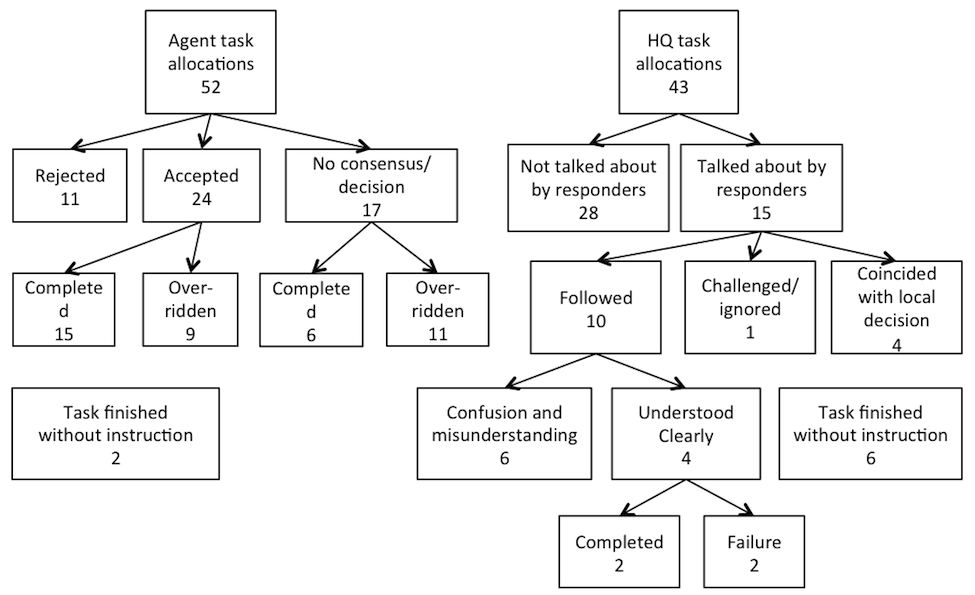
\includegraphics{message_handling.png}
\vspace{-5mm}
\caption{How task allocations were handled by first responders in the version with agent (left), and without agent (right).\vspace{-3mm}}\label{fig:msgs}
\end{figure}

In contrast, when task allocation was handled by the agent (52 tasks allocated in two trials on average), responders explicitly accepted 24 tasks,  of which they completed 15  successfully. Although there was either no response or no consensus between the responders (in 17 tasks allocated), they still completed 6 of these tasks successfully. In total, 20 task allocations were withdrawn by the agent as a result of re-planning. 



%\paragraph{Rejecting task allocations}
In terms of task rejections, first responders rejected $PA$'s task allocation 11 times in the agent version. All of the rejections happened when the task allocation would have \emph{split existing teams}, or instructed responders to team up with \emph{physically more distant responders}. In most cases (9 out of 11), they triggered re-planning by rejection and \emph{adjusted the task allocation} to become consistent with the responder's current team. In the other two cases, the responders rejected  the task allocation one more time before receiving the desired task allocation. For accepted instructions, the average distance between suggested teammates was 12 metres. For rejected instructions, the average was 86 metres.

The results above show that  the simple mechanism to get $PA$ to re-plan (i.e., reject/accept) was more successful (more tasks completed and less confusion) than the open-ended interactions between $H$ and the responders (that were open to confusion).  Moreover, the fact that many of the rejections were due to the long distance to travel and teammate preference, implies that players chose to do the tasks they \emph{preferred}  rather than those deemed optimal by the agent. This indicates there may be an issue of trust in the agent, but also that it may be easier for a responder  to impose (through a reject) such preferences on an agent (and indirectly to other team members) rather than expressing this to $H$ or directly to teammates. 
% Role of HQ commander
It is also important to note that in the agent-assisted setting, $H$ frequently \emph{monitored} the allocation of tasks  returned by the agent (57 clicks on `show task' in UI responder status widget). Whereas 43 directives out of 68 in the non-agent session were task allocations, only 16 out of 68 were directly related to task allocations in the agent version. Out of these, $H$ directly reinforced the agent's instruction 6 times (e.g., ``SS and LT retrieve 09''), and complemented (i.e., added to or elaborated) $PA$'s task allocation 5 times (e.g., ``DP and SS, as soon as you can head to 20 before the radiation cloud gets there first''). $H$  did `override' $PA$'s instruction in 5 cases.  

In the agent version, most of $H$'s directives (52 out of 68) and assertives (49 out of 51) focussed on providing situational awareness and  routing the responders to avoid exposing them to radiation. For example, ``NK and JL approach drop off 6 by navigating via 10 and 09.'', or ``Radiation cloud is at the east of the National College''. 

%\subsubsection{Summary and Guidelines}\label{sec:summary}
In summary, these results suggest three key observations with regard to  human-agent coordination in the trial: 
\begin{enumerate}
\item First responders performed better (rescued more targets)  and maintained higher health levels when supported by the agent.  These results echo those obtained under simulation (see Section \ref{sec:algo}) and  may reflect the better forward-planning capability of the planning agent compared to human responders. 
 
\item Rejecting tasks was relatively frequently employed to trigger re-planning to obtain new task allocations aligned with responder preferences.  In each case, the planning agent was able to adapt to provide an alternative  that was acceptable to the responders. Without this facility we believe the responders would have chosen to ignore the plan. Task rejection seemed to be linked to changes to established teams, especially when members were relatively distant. Consequently, these kinds of allocations may need particularly support (e.g., explanation) or might be less preferentially selected by $PA$.

\item When task allocation was handled by $PA$, $H$ could focus on providing vital situational awareness to safely route first responders around danger zones: thus demonstrating effective division of labour and complementary collaboration between humans and agents.
\end{enumerate}

Given the above observation we argue that a planning agent for team formation should not only model the uncertainty in player behaviours and in the environment, but that interactional challenges also need to be addressed  if such a technology is to be accepted in practice. In particular, we propose the following design guidelines for human-agent collaborations:\\

\noindent \textbf{Adaptivity}: our experiences suggest that planning algorithms should be designed to take in human input, and more importantly, be \emph{responsive} to the needs of the users. As we saw in AtomicOrchid, players repeatedly requested new tasks and this would not have been possible unless our algorithm  was computationally efficient but could dynamically assimilate updates, requests, and constraints dynamically. We believe this makes the algorithm more acceptable to the users.\\

\noindent \textbf{Interaction Simplicity}: our agent was designed to issue simple commands (Do X with Y) and respond to simple requests (OK or Reject Task). Such simple messages were shown to be far more effective at guiding players to do the right task than the unstructured human communication in the non-agent assisted case that was fraught with inconsistencies and inaccuracies. In fact, we would suggest that agents should be designed with minimal options to simplify the reasoning users have to do to interact with the agent, particularly when they are under pressure to act.\\

\noindent \textbf{Flexbile autonomy}: the HQ dashboard proved to be a key tool for the HQ coordinator $H$ to \emph{check} and \emph{correct for} the allocations of $PA$, taking into account the real-world constraints that the players on the ground faced. In particular, letting the human oversee the agent (i.e., ``on-the-loop") at times and actively instructing  the players (and bypassing the agent) at other times (i.e., ``in-the-loop") as and when needed, was seen to be particularly effective. This was achieved by $H$ \emph{without the agent} defining when such transfers of control should happen (as in \cite{scerri:etal:2005}) and, therefore, left the coordinator the option of taking control when she judged it was needed. Hence, we suggest that such deployed autonomous systems should be built for flexible autonomy. Specifically, interfaces should be designed to pass control \emph{seamlessly} between humans and agents.


